\chapter{Graphs}\label{cha:graphs}

Here be graphs.

\section{Learning Curves}\label{sec:learning_curves}

Learning curves plots the evaluation metric with respect to a varying training set size. Evaluated with a top-10 recommender list, using F-measure.

\textit{x-axis should it be training size or percent?}

\begin{itemize}
    \item alpha
    \item alpha2
    \item eswc2015movies
    \item eswc2015music
    \item eswc2015books
    \item movielens1m
    \item romeo
\end{itemize}

\Warning[TODO]{ Generate better graphs!! }
\Warning[TODO]{ Why predetermined? Title is WRONG! }


\begin{figure}[ht]
  \centering
    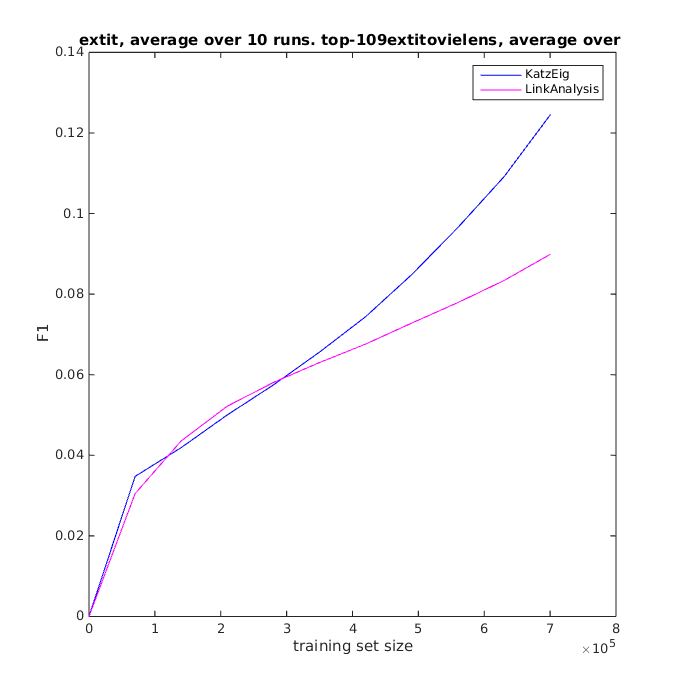
\includegraphics[width=0.9\textwidth]{fig/learning_curves/movielens_learning_curves.png}
    \caption{Learning curves using \textit{movielens1m}
        Used a predetermined $\eta = -2$ and $\gamma = 1.8$ for link-analysis and $\beta = \frac{1}{|A_{train}|}$ with the model $K = 30$ for katz-eig.}
  %\label{fig:sysoverview}
\end{figure}

\begin{figure}[ht]
  \centering
    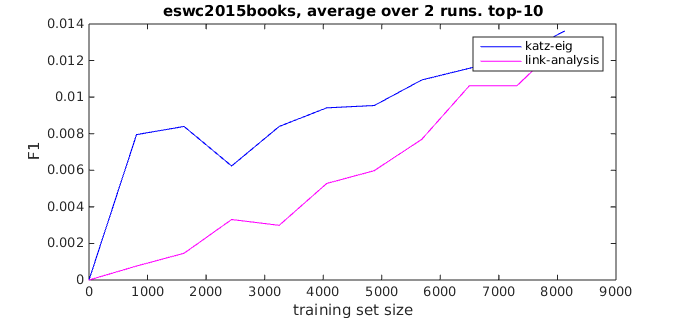
\includegraphics[width=0.9\textwidth]{fig/learning_curves/eswc2015books_learning_curves.png}
    \caption{Learning curves using \textit{eswc2015books}
        Used a predetermined $\eta = -2$ and $\gamma = 1.8$ for link-analysis and $\beta = \frac{1}{|A_{train}|}$ with the model $K = 30$ for katz-eig.}
  %\label{fig:sysoverview}
\end{figure}


%Used a predetermined $\eta = -2$ and $\gamma = 1.8$ for link-analysis and $\beta = \frac{1}{|A_{train}|}$ with the model $K = 10$ for katz-eig.


XXX link-analysis is slower the more training data we have.
katz-eig is practically indifferent.
plot time!

\FloatBarrier


\section{Training Curves}\label{sec:training_curves}

Training curves plots the evaluation metric, or error estimation, with respect to epochs, the number of iterations in an iterative algorithm.

\subsection{katz-eig}

\begin{itemize}
    \item alpha
    \item alpha2
    \item eswc2015movies
    \item eswc2015music
    \item eswc2015books
    \item movielens1m
    \item romeo
\end{itemize}


\subsection{link-analysis}

\begin{itemize}
    \item alpha
    \item alpha2
    \item eswc2015movies
    \item eswc2015music
    \item eswc2015books
    \item movielens1m
    \item romeo
\end{itemize}


\section{katz-eig}
\Warning[TODO]{ title? Where? What? How? :) }

Also final runtime to find beta/K for different datasets

\subsection{$\beta$}

XXX For what K? Different K? Best K?

\begin{itemize}
    \item alpha
    \item alpha2
    \item eswc2015movies
    \item eswc2015music
    \item eswc2015books
    \item movielens1m
    \item romeo
\end{itemize}


\subsection{$K$}

XXX For what beta? Search every iteration?

\begin{enumerate}
    \item K / F-measure
    \item K / running time
\end{enumerate}

\begin{itemize}
    \item alpha
    \item alpha2
    \item eswc2015movies
    \item eswc2015music
    \item eswc2015books
    \item movielens1m
    \item romeo
\end{itemize}


\section{link-analysis}
\Warning[TODO]{ title? Where? What? How? :) }

\begin{enumerate}
    \item Plot the whole function space (limited ofc)
    \item Scatter table with randomized large values
\end{enumerate}

\subsection{$\gamma$}

\subsection{$\eta$}


\section{Big comparisons?}
\Warning[TODO]{ title? Where? What? How? :) }

Compare katz-eig, link-analysis, and some other algorithm?
Also compare optimization w.r.t. time and evaluation.

\begin{enumerate}
    \item Running time
    \item F-measure
\end{enumerate}

